\documentclass[10pt]{article}

\usepackage{times}
\usepackage{graphicx}
\usepackage{subfigure}
\usepackage{natbib}
\usepackage{algorithm}
\usepackage{algorithmic}
\usepackage{lipsum}
\usepackage{todonotes}
\usepackage[accepted]{icml2017}

\usepackage{macros}


\newcommand{\bert}{\operatorname{BERT}}
\newcommand{\distortion}{\operatorname{Distortion}}
\newcommand{\prune}{\operatorname{Prune}}
\newcommand{\diffprune}{\operatorname{DiffPrune}}
\newcommand{\rankreduce}{\operatorname{RankReduce}}


\newcommand{\btheta}{{\bm{\theta}}}
\newcommand{\bphi}{{\bm{\phi}}}
\newcommand{\bpsi}{{\bm{\psi}}}
\newcommand{\bvartheta}{{\bm{\vartheta}}}


\icmltitlerunning{BERT Model Compression and Weight Sharing}

\begin{document}

\twocolumn[
\icmltitle{BERT Model Compression and Weight Sharing}
\begin{icmlauthorlist}
  \icmlauthor{Jiafeng Chen}{}
\icmlauthor{Yufeng Ling}{}
\icmlauthor{Francisco Rivera}{}
\end{icmlauthorlist}

\vskip 0.3in
]

\begin{abstract}
\raggedright
  \begin{itemize}
  \item We apply model compression techniques to fine-tuned BERT on multiclass
  classification problems.
  \item Knowledge distillation and DeepTwist-based compression techniques give
  us moderate compression benefits for a commensurate decrease in model
  performance.
  \item We achieve our most compelling results from employing the DeepTwist
  framework to share weights across BERT models fine-tuned for different tasks.
  \item Our work demonstrates most weights need not change in the fine-tuning
  process.
%   \item This document describes the expected style, structure, and rough
%   proportions for your final project write-up.
%   \item While you are free to break from this structure, consider it a strong
%   prior for our expectations of the final report.
%   \item Length is a hard constraint. You are only allowed max \textbf{8 pages}
%   in this format. While you can include supplementary material, it will not be
%   factored into the grading process. It is your responsibility to convey the
%   main contributions of the work in the length given.
  \end{itemize}



\end{abstract}

\section{Introduction}
\label{sec:introduction}

% Example Structure:
% \begin{itemize}
% \item What is the problem of interest and what (high-level) are the current best methods for solving it?
% \item How do you plan to improve/understand/modify this or related methods?
% \item Preview your research process, list the contributions you made, and summarize your experimental findings.
% \end{itemize}

Deep Neural Networks (DDNs) have become the state-of-art for many tasks in
language modeling. At the same time, they have become progressively larger in
size, due to both larger out-of-box pre-trained embeddings and deeper
networks. However, in order to deploy the models on more resource-constrained
devices, such as mobile devices or even older personal laptops, as opposed to
on cloud virtual machines, it is crucial to reduce the size of the models.

Previous work has had a lot of success in computer vision tasks.
\citet{han2015deep} was able to combine pruning, quantization and Huffman
coding to reduce the size of AlexNet by 35$\times$ and the size of VGG-16 by
49$\times$ without loss of accuracy. Recently, similar compression techniques
were applied by \citet{cheong2014transformer} on language models, Transformers
in specific, and reduced the size by a factor of 5.85 while retaining 98.43\%
of the performance. To the best of our knowledge, compressing language models
still remains an under-studied field.

In this paper, we demonstrate that the DeepTwist framework
\citep{lee2018deeptwist} is applicable to compressing fine-tuned BERT
\citep{devlin2018bert} on multiclass classification problems in addition to
computer vision tasks, though the drop in performance is less negligible.
Knowledge distillation also achieves the compression objective with more than
desired decrease in predictive accuracy.

We used two of the GLUE datasets SST-2 and QQP. We ran most of the experiments
on SST-2, a binary sentiment classification task on single-sentence movie
reviews. We validated the results on QQP, a binary classification task for
whether two questions asked on Quora are semantically equivalent.

The most important contribution of this paper is that we proposed a new
weight-sharing method called ``Difference Pruning'' which imposes constraint on
the sparcity of weight difference with the pre-trained BERT model. While
uncompressed fine-tuned BERT model achieves 92.9\% validation accuracy on
SST-2, the Difference Pruning model that keeps 99\% of the pre-trained BERT
weights achieves 91.3\% on the validation set. This enables multiple language
modeling tasks to share the weights of pre-trained BERT and each incurs minimal
extra storage space requirements.

\section{Background}

% Example Structure:
% \begin{itemize}
% \item What information does a non-expert need to know about the problem domain?
% \item What data exists for this problem?
% \item What are the challenges/opportunities inherent to the data? (High
% dimensional, sparse, missing data, noise, structure, discrete/continuous,
% etc?)
% \end{itemize}

DNNs have become extremely large in size with growing complexities. A BERT
base model has 110M parameters and takes 438 MB disk space to store. This
makes it very hard to deploy those models on mobile devices, which in most
cases have limited storage and RAM and low computational resources. As a
result, we are not able to store multiple models for different tasks on mobile
devices. Allocating hundreds of megabytes to to those models is also not
realistic for mobile apps such as Gmail or Facebook. And due to increasing
privacy concerns, users prefer models generating predictions based on their
input to be running locally instead of sending information to the cloud. Last
but not least, evaluating enormous models takes too much time on mobile
devices and can drain batteries significantly.

The challenge that we are facing is therefore how to compress DNNs in size
while keeping their predictive performance competitive with full model.


\section{Related Work}

% Example Structure:
% \begin{itemize}
% \item What 3-5 papers have been published in this space?
% \item How do these  differ from your approach?
% \item What data or methodologies do each of these works use?
% \item How do you plan to compare to these methods?
% \end{itemize}

We are interested in compressing the language representation model BERT
\citep{devlin2018bert}.  It is the state-of-art result in many natural
language processing tasks  such as natural language inference, paraphrasing
and named entity recognition.

\citet{cheng2017survey} provides a comprehensive overview of the state-of-art
methods to compress DNNs. Of the methods summarized by the paper, the ones
that are of interest to our work are weight-pruning and quantization
\citep{han2015deep}, and low-rank factorization \citep{denton2014exploiting}.
Knowledge distillation, first proposed by \citep{bucilua2006model} as
``knowledge transfer'', was recently popularized by
\citep{hinton2015distilling}. It differs from the previously mentioned methods
since it compresses an existing model by replacing it with a simpler model
that is trained on its outputs.

DeepTwist, a end-to-end training framework, allows us to incorporate
compression procedures into training \citep{lee2018deeptwist}. Under this
framework, the model parameters are occasionally distorted during training
time instead of only at the end. This framework has the benefit of simplified
training procedure and faster convergence and reduced requirement for
hyperparameter tuning. Experiment on MNIST dataset with DeepTwist shows that
LeNet-5 and LeNet-300-100 models are able to retain predictive accuracy under
high compression rate.


\section{Inference (or Training)}
\label{sec:training}


\subsection{Knowledge Distillation}
\label{subsec:kd}

In this paper, we limit our purview to text classification tasks. Training
neural-network-based systems for this task typically consists of a form of
gradient descent based on a differentiable loss function which takes in the
prediction for a given example and the correct label. That is, if we have
training data $(\bm{x}_i, y_i)$ and model $f$, we would aim to minimize,
\[ \ell(f(\bm{x_i}), y_i)\]
where usually the loss function is taken to be Cross-Entropy loss. When we
already have a model $f$ that performs well, we can leverage this training
paradigm through a modification called \emph{knowledge distillation}. Given
the large model that performs well, termed the \emph{teacher network}, we
train a smaller network $g$, the \emph{student network}, by minimizing,
\[ \ell(g(\bm{x_i}), f(\bm{x_i})).\]
Here, we can no longer use Cross-Entropy loss because $f(\bm{x}_i)$ is a
probability distribution rather than a specific label. However, we can take
$\ell$ to be either mean-square error (MSE) between the probabilities in
log-space, or Kullback-Leibler (KL) loss. We avoid MSE error on the
probabilities themselves because of disappearing gradients when the predicted
probabilities are very close to 0 or 1.

The benefits of training in this fashion have been empirically documented
\citep{hinton2015distilling} and have theoretical motivation. Our goal of any
network is to learn the conditional distribution 
\[ p(y_i = k \mid \bm{x}_i).\]
In traditional training, we do this by observing the draws $y_i$ from this
distribution. However, to the extent that the teacher network prediction is a
good approximation of the true conditional distribution, the student network
can learn faster because it is being pushed toward predicting the de-noised
expectation.

To present a simplified example: if a neural network were trying to understand
a coin flip, it would require a number of observations of heads and tails to
conclude the underlying probability is 50\% toward either direction. However,
if it is directly shown that the probability was 50\% each time, regardless of
what the coin came up, it will in less time understand that the probability is
always 50\%.

An additional benefit from knowledge distillation arises from BERT's
pre-training. Because BERT is pre-trained on large amounts of unstructured
data, it contains a powerful language model which likely would be impossible
to learn from the specific task's data-set. To an extent, relevant features
from this language model are what make BERT so powerful once it's fine-tuned.
Training the student network on BERT's output thus allows some of this
``outside knowledge'' to percolate toward the student network.

To provide a concrete example of how this might work, suppose BERT captures
from its pre-training that ``bad'', ``horrible,'' and ``terrible'' are
approximate synonyms. In a sentiment task, these three words appear in three
different sentences, two of which are negative, and one of which is positive.
A fine-tuned BERT may predict a lower likelihood of being positive to the
positive sentence than it would otherwise even if the word of interest appears
nowhere else.

For our knowledge distillation, we make use of a fine-tuned BERT on a task as
our teacher network and train a simpler model to emulate the predictions. For
the student network, we use both a CNN and an LSTM, specified further in
\cref{sec:model}.

\subsection{Deep Twist}

Knowledge distillation operates by passing knowledge from a teacher network to a
student network. There is no requirement that these networks resemble each other
in any way. We may, however, wish to directly compress a model whose
architecture we've had success with.

To this end, we follow the framework put forward by \citet{lee2018deeptwist},
\emph{DeepTwist}, whose training loop is characterized by \cref{algo:deeptwist}.
Training of the model closely resembles SGD with one important modification:
every $S_d$ batches, the model weights are transformed by a \emph{distortion}
function. 

\begin{algorithm}
  \begin{algorithmic}
    \STATE{$n \leftarrow$ number of batches per epoch}
    \STATE{$\theta \leftarrow$ initialization of model parameters}
    \STATE{$k \leftarrow$ number of epochs to train}
    \STATE{$S_d \leftarrow$ distortion step}
    \FOR{$i=0$ to $k \cdot n$}
      \STATE{batch $\leftarrow$ batches[$i \pmod n$]}
      \STATE{$\theta \leftarrow \theta - \eta \nabla \ell(\theta,
      \text{batch})$}
      \COMMENT{gradient step}
      \IF{$i \equiv 0 \pmod{S_d}$}
        \STATE{$\theta \leftarrow \distortion(\theta)$}
      \ENDIF
    \ENDFOR
    \STATE{$\theta \leftarrow \distortion(\theta)$}
  \end{algorithmic}
  \caption{DeepTwist Training Loop}
  \label{algo:deeptwist}
\end{algorithm}

We have significant flexibility in picking a distortion function, but in order
to be useful, it must provide compression benefits. That is, the image of the
distortion function should have a parameterization that takes less space in
memory than then range of all possible $\theta$s. For example, if $\theta \in
\mathbb{R}^{m,n}$, and the distortion produces a matrix of rank 1, then any
distorted matrix could be uniquely identified by $\theta' \in \mathbb{R}^{n+m}$
through a matrix factorization.

It is important to note that while $\theta$ will be compressible immediately
after a distortion step, there is no guarantee that it will remain so after some
gradient steps. In fact, almost surely it will not be. Thus, we also enforce
that the process ends on a distortion step.

\section{Model}
\label{sec:model}

We first set up some notation. Let $F_\btheta = G_\bpsi \circ \bert_\bphi$ be
a transformed model where $\btheta = (\bphi, \bpsi)$ be parameters of the
subparts of the model. $\bert_\bphi$ is a BERT model where the pretrained
weights are $\bphi_0 = (\bphi_0^i)_{i=1}^n$, and $G_\bpsi$ is additional
layers for fine-tuning BERT, parameterized by $\bpsi$. We decompose the
subparts of the model into layers: \begin{align*}
\bert_\bphi &= f_{n}^{\bphi_n} \circ \cdots \circ f_1^{\bphi_1} \\
G_\bpsi &= g_{m}^{\bpsi_m} \circ \cdots \circ g_1^{\bpsi_1}.
\end{align*}

% \subsection{DeepTwist-based Weight Distortions}


Given training data $(\bm x_i, y_i)_{i=1}^N$, where $\bm x_i$ are one-hot
encoded tokens, we train by solving the standard maximum likelihood problem
where \[
\min_{\btheta} \sum_{i=1}^N \ell\pr{y_i, F_\btheta(\bm x_i)}
\]
for some loss function specific to the task. For instance, $\ell$ is
cross-entropy loss for a (multiclass) classification problem, and $\ell$ is
mean-squared-error for a regression problem, which correspond to
log-likelihoods in Categorical and Gaussian models, respectively. The
innovation of DeepTwist-based training is perturbing the usual gradient-based
optimization by repeatedly distorting the current weights to achieve
compression objectives.

Specifically, the DeepTwist framework presented in \Cref{sec:training} applies
a distortion step for fixed intervals during training, where \[
\btheta \gets \distortion(\btheta). 
\]
In this section, we discuss a few methods for parameterizing $\distortion$.
Generally, we may imagine a few special cases of distortion, we call a
particular distortion \emph{distortion by layer} if it is applied per layer,
i.e. \begin{align*}
\distortion'(\btheta) &= \\
(&\distortion(\bphi_1),\ldots,\distortion(\bphi_n),\\
&\distortion(\bpsi_1),\ldots, \distortion(\bpsi_m)).
\end{align*}
We call a particular distortion \emph{pretrained-only} if \[
\distortion'(\btheta) = \distortion(\bphi).
\]

We list a few methods of parameterizing the distortion step. 
\paragraphdot{Pruning} Consider a parameter vector $\bvartheta$, let
  $t_p$ be the $p$-th quantile of the vector $\bvartheta$. Then \[
  \prune(\bvartheta; p) = \one(|\bvartheta| > t_p) \odot \bvartheta
  \]
  be the vector where values in $\bvartheta$ below $t_p$ are zeroed. 
  
  Pruning is an extremely simple procedure. When $p$ is large, say, $p=0.99$,
  we may take advantage of sparsity of the resulting model by saving locations
  of nonzero entries, and thus reducing the model size in memory. However,
  such compression does not come without potential sacrifices to computational
  speed, as computation needed to be carried out on sparse data structures,
  which may not effectively make use of standard hardware.
  
  Pruning is an out-of-the-box procedure that works with any models. However,
  as a price of the generality, pruning fails to be tailored to the nature of
  BERT being a pre-trained model. Suppose the pretrained weights $\bphi_0 $
  capture certain structure of language, then dramatic distortions to
  $\bphi_0$ essentially discards the information, especially early in the
  training loop. We may partially remedy this issue by either using a dynamic
  pruning rate, where pruning rate is small early in the training loop or by
  using layer-specific pruning rates, with layers in $\bert$ having a lower
  pruning rate than layers in $G$. 
  
  A direct approach to taking advantage of pretrained models, however, is
  \emph{difference pruning}, where we ensure that the difference between the
  model and a pretrained model is sparse. Effectively, difference pruning
  ensures a form of weight sharing between various BERT-based models for
  different tasks.
  
\paragraphdot{Difference Pruning} Consider some pretrained weights
$\bvartheta_0$, define \[
\diffprune(\bvartheta; \bvartheta_0, p ) = \bvartheta_0 + \prune(\bvartheta -
\bvartheta_0 ; p). 
\]
Observe that difference pruning provides no compression benefits when there is
only one fine-tuning task; however, when the number of potential tasks is
large, we only need to save $\btheta_0$ and the sparse matrix $\btheta -
\btheta_0,$ and $\btheta_0$ is shared across tasks.

Observe that we can transform any reduction technique by applying the
reduction technique on the difference, and thus the \emph{difference} should
be viewed (and is implemented) as a decorator to a conventional distortion
technique.


\paragraphdot{Rank Reduction} If $\bvartheta$ is a matrix, then we may apply
rank
reduction via singular value decomposition \[
\bvartheta = U\Sigma V^\top
\]
where $\Sigma$ is a diagonal matrix, where $U \in \R^{n\times n}, \Sigma\in \R^
{n\times n}, V\in \R^{m\times n}$, and $\bvartheta \in \R^{n\times m}$.

We distort via \[
\rankreduce(\bvartheta; r) = \tilde U \tilde \Sigma \tilde V^\top,
\]
where $\tilde U, \tilde \Sigma, \tilde V$ are conforming matrices such that the
smallest values on the spectrum $\Sigma$ is zeroed out, as well as corresponding
values in $U,V$. If we keep only the $r$ largest spectral values, then we store
$\tilde U \tilde \Sigma$, an $n\times r$ matrix, and $\tilde V$, an $m\times r$
matrix. Thus, instead of storing $2nm$ floats, we may store $r(n+m)$, achieving
a compression rate of \[
\rho = \frac{r(n+m)}{2mn}.
\]
Note however, that storing matrices in this manner requires an additional
matrix multiplication in evaluation time, since we have to compute the product
$\tilde U \tilde \Sigma \tilde V$.

% \subsection{Knowledge Distillation}


% Example Structure:

% \begin{itemize}
% \item What is the formal definition of your problem?
% \item What is the precise mathematical model you are using to represent it? In
% almost all cases this will use the probabilistic language from class, e.g.
%   \begin{equation}
%   z \sim {\cal N}(0, \sigma^2)\label{eq:1}
% \end{equation}
% But it may also be a neural network, or a non-probabilistic loss,
% \[ h_t \gets \mathrm{RNN}(x_{t}, h_{t-1} )\]

% This is also a good place to reference a diagram such as Figure~\ref{fig:diagram}.

% \item What are the parameters or latent variables of this model that you plan
% on estimating or inferring? Be explicit. How many are there? Which are you
% assuming are given? How do these relate to the original problem description?
% \end{itemize}



% \begin{figure}
%   \centering
%   \missingfigure[figheight=8cm]{}
%   \caption{\label{fig:diagram} This is a good place to include a diagram
%   showing how your model works. Examples include a graphical model or a neural
%   network block diagram.}
% \end{figure}

% \subsection{Knowledge Distillation}


% Example Structure:

% \begin{itemize}
% \item What is the formal definition of your problem?
% \item What is the precise mathematical model you are using to represent it? In
% almost all cases this will use the probabilistic language from class, e.g.
%   \begin{equation}
%   z \sim {\cal N}(0, \sigma^2)\label{eq:1}
% \end{equation}
% But it may also be a neural network, or a non-probabilistic loss,
% \[ h_t \gets \mathrm{RNN}(x_{t}, h_{t-1} )\]

% This is also a good place to reference a diagram such as Figure~\ref{fig:diagram}.

% \item What are the parameters or latent variables of this model that you plan
% on estimating or inferring? Be explicit. How many are there? Which are you
% assuming are given? How do these relate to the original problem description?
% \end{itemize}



% \begin{figure}
%   \centering
%   \missingfigure[figheight=8cm]{}
%   \caption{\label{fig:diagram} This is a good place to include a diagram
%   showing how your model works. Examples include a graphical model or a neural
%   network block diagram.}
% \end{figure}




\section{Methods}
In this section, we briefly discuss our experimental setup. We mostly
work with
SST-2, a binary sentiment classification task in the GLUE multitask benchmark
framework \citep{wang2018glue}. We also validate the model's
performance with trial on the Quora Question Pair (QQP) task, which is a
binary classification task for whether two questions are equivalent. We
train with a maximum sequence length of 64 and batch size of 32 on the
NC-6 and NC-12 virtual machines on Microsoft Azure. We use the basic 
\texttt{BERT-base-uncased} model for our experimental results. We employ
early stopping in training, with patience of 1 epoch, and early stopping is
guided by validation error. 

\subsection{DeepTwist}
We implement the DeepTwist framework with default frequency of distortion
every 10 batches. Additionally, we ensure that training ends on a
distortion step, so that the model produced by training has compression
benefits. For $\prune$ and $\diffprune$ distortions, we use a single
pruning rate held fixed throughout training. 


\subsection{Knowledge Distillation}

For knowledge distillation experiments, we use various configurations of the
student network: \paragraphdot{LSTM} We use a one-layer LSTM network with hidden
dimension $H=200$. We first embed the one-hot representation of tokens, and we
feed the embeddings through an LSTM. We then map the last hidden state of the
LSTM through a linear layer for classification.  \paragraphdot{CNN} We use an
implementation\footnote{\url{https://github.com/jfilter/cnn-text-classification-pytorch/blob/master/cnn_text_classification/model.py}}
of \citet{kim2014convolutional} with kernel sizes $(3,4,5)$, hidden size
$H=300$, no dropout, and $20$ kernels for each kernel size.\footnote{These are
default in the implementation we used.} 

For each model, we initialize the embedding layer of the model with the
first $H$ dimensions of the corresponding embedding layer in pretrained
BERT. 



\section{Results}

\begin{itemize}
\item What were the results comparing previous work / baseline systems / your
systems on the main task?
\item What were the secondary results comparing the variants of your system?
\item This section should be fact based and relatively dry. What happened, what
was significant?
\end{itemize}

% \begin{table*}
%   \centering
%   \missingfigure{}
%   \caption{This is usually a table. Tables with numbers are generally easier
%   to read than graphs, so prefer when possible.}
%   \label{fig:mainres}
% \end{table*}


% \begin{table}[tbh]
%         \caption{Results for DeepTwist}
%         \label{tab:deeptwist_results}
%         \centering
%         \vspace{1em}
%         \begin{tabular}{lccccc}
% \toprule
% {} &               type &  param &  val loss &   val acc \\
% {} & 
% \hypertarget{tabcol:1}{(1)} & \hypertarget{tabcol:2}{(2)} & \hypertarget{tabcol:3}{(3)} & \hypertarget{tabcol:4}{(4)} \\ \midrule
% 0  &  diff prune global &   $90$ &   $0.211$ &   $0.912$ \\
% 1  &              prune &   $20$ &   $0.291$ &   $0.886$ \\
% 2  &              prune &   $80$ &   $0.532$ &   $0.767$ \\
% 3  &         diff prune &   $80$ &   $0.222$ &   $0.916$ \\
% 4  &  diff prune global &   $99$ &       --- &       --- \\
% 5  &  diff prune global &   $90$ &   $0.213$ &   $0.916$ \\
% 6  &         diff prune &   $40$ &   $0.203$ &   $0.909$ \\
% 7  &                svd &   $50$ &   $0.490$ &   $0.810$ \\
% 8  &                svd &  $200$ &   $0.459$ &   $0.845$ \\
% 9  &              prune &   $40$ &   $0.424$ &   $0.845$ \\
% 10 &              prune &   $60$ &   $0.425$ &   $0.815$ \\
% 11 &  diff prune global &   $99$ &   $0.230$ &   $0.901$ \\
% 12 &  diff prune global &   $99$ &   $0.222$ &   $0.905$ \\
% 13 &         diff prune &   $99$ &   $0.222$ &   $0.913$ \\
% 14 &         diff prune &   $95$ &   $0.221$ &   $0.916$ \\
% 15 &         diff prune &   $90$ &   $0.216$ &   $0.916$ \\
% 16 &         diff prune &   $60$ &   $0.209$ &   $0.920$ \\
% 17 &                svd &  $100$ &   $0.515$ &   $0.823$ \\
% 18 &                svd &  $150$ &   $0.456$ &   $0.828$ \\
% 19 &         diff prune &   $80$ &   $2.533$ &   $0.491$ \\
% 20 &         diff prune &   $90$ &       --- &       --- \\
% 21 &  diff prune global &    $0$ &   $0.738$ &   $0.509$ \\
% 22 &         diff prune &    $0$ &   $0.692$ &   $0.522$ \\
% 23 &         diff prune &    $0$ &   $1.854$ &   $0.491$ \\
% \bottomrule
% \end{tabular}

% \end{table}

\newlength{\tableblocksep}
\setlength{\tableblocksep}{1ex}

\begin{table}[tbh]
        \caption{DeepTwist SST-2 Results}
        \label{tab:deeptwistresults}
        \centering
        \vspace{1em}
        \begin{tabular}{p{1ex}lcccc}
\toprule
& &       Val. Loss & Val. Acc. \\
\cmidrule{3-4}
\multicolumn{2}{l}{Uncompressed BERT} & $0.266$ & $92.9\%$ \\[\tableblocksep]
\multicolumn{2}{l}{Diff.\ Pruning} \\
& $p=40\%$  & $0.203$ & $90.9\%$ \\
& $p=60\%$  & $0.209$ & $92.0\%$ \\
& $p=80\%$  & $0.222$ & $91.6\%$ \\
& $p=90\%$  & $0.216$ & $91.6\%$ \\
& $p=95\%$  & $0.221$ & $91.6\%$ \\
& $p=99\%$  & $0.222$ & $91.3\%$ \\
& $p=100\%$ & $0.692$ & $52.2\%$ \\[\tableblocksep]
\multicolumn{2}{l}{Diff.\ Pruning (global)} \\
& $p=90\%$  & $0.213$ & $91.6\%$ \\
& $p=99\%$  & $0.222$ & $90.5\%$ \\
& $p=100\%$ & $0.738$ & $50.9\%$ \\[\tableblocksep]
\multicolumn{2}{l}{Pruning} \\
& $p=20\%$  & $0.291$ & $88.6\%$ \\
& $p=60\%$  & $0.425$ & $81.5\%$ \\
& $p=40\%$  & $0.424$ & $84.5\%$ \\
& $p=80\%$  & $0.532$ & $76.7\%$ \\[\tableblocksep]
\multicolumn{2}{l}{SVD} \\
& $r=200$   & $0.459$ & $84.5\%$ \\
& $r=150$   & $0.456$ & $82.8\%$ \\
& $r=100$   & $0.515$ & $82.3\%$ \\
& $r=50$    & $0.490$ & $81.0\%$ \\[\tableblocksep]
\bottomrule
\end{tabular}

        \end{table}


\begin{table}[tbh]
        \caption{Knowledge Distillation SST-2 Results}
        \label{tab:kd_results}
        \centering
        \vspace{1em}
        \begin{tabular}{p{.1em}lcccc}
\toprule
& & \multicolumn{2}{c}{No KD} & \multicolumn{2}{c}{KD} \\
\cmidrule(lr){3-4} \cmidrule(lr){5-6}
& & Val. Loss & Val. Acc & Val. Loss & Val. Acc \\
\cmidrule{3-6}
\multicolumn{2}{l}{LSTM} & $0.513$ & $80.5\%$ & $0.738$ & $83.1\%$ \\[\tableblocksep]
\multicolumn{2}{l}{CNN}  \\
& $d=0$ & $0.426$ & $81.2\%$ & $0.423$ & $83.4\%$ \\
& $d=0.5$ & $0.418$ & $82.8\%$ & $z$ & $a$ \\
\bottomrule
\end{tabular}

\end{table}


% \begin{table}[tbh]
%         \caption{Results for Knowledge Distillation}
%         \label{tab:kd_results}
%         \centering
%         \vspace{1em}
%         \begin{tabular}{lccccccc}
% \toprule
% {} &  framework &  type &  val loss &  ß val acc \\
% {} & \hypertarget{tabcol:1}{(1)} & \hypertarget{tabcol:2}{(2)} & \hypertarget{tabcol:3}{(3)} & \hypertarget{tabcol:4}{(4)} \\
% \midrule
% 0 &        nokd &   CNN &   $0.906$ &   $0.799$ \\
% 1 &        nokd &   CNN &   $0.448$ &   $0.784$ \\
% 2 &        nokd &   CNN &   $0.856$ &   $0.812$ \\
% 3 &          kd &  LSTM &   $0.738$ &   $0.831$ \\
% 4 &          kd &   CNN &   $0.423$ &   $0.834$ \\
% \bottomrule
% \end{tabular}
% \label{tbl:kdresults}
% \end{table}

\section{Discussion}

Our most striking result is the robust performance of difference pruning. Even
keeping upwards of 99\% of the weights unchanged gives us performance that is
very competitive with the unrestricted model. Most of our experiments are on
SST-2, but we see success with this method on QQP as well, suggesting that
small changes to pre-trained BERT are sufficient for performance on a specific
task. 

As expected, pruning a higher proportion of the weights decreases performance,
but we are happily surprised at the relatively low magnitude of this effect even
at high prune rates. Pruning with a global threshold rather than in a
stratified way produces distinctly worse results. We suspect this is due to
weights in different layers having different magnitudes, making a global
threshold have an undue effect on layers whose weights tend to be smaller. We
confirm this heterogeneity in \cref{fig:weightsbylayer}.

\begin{figure}[htb]
\centering
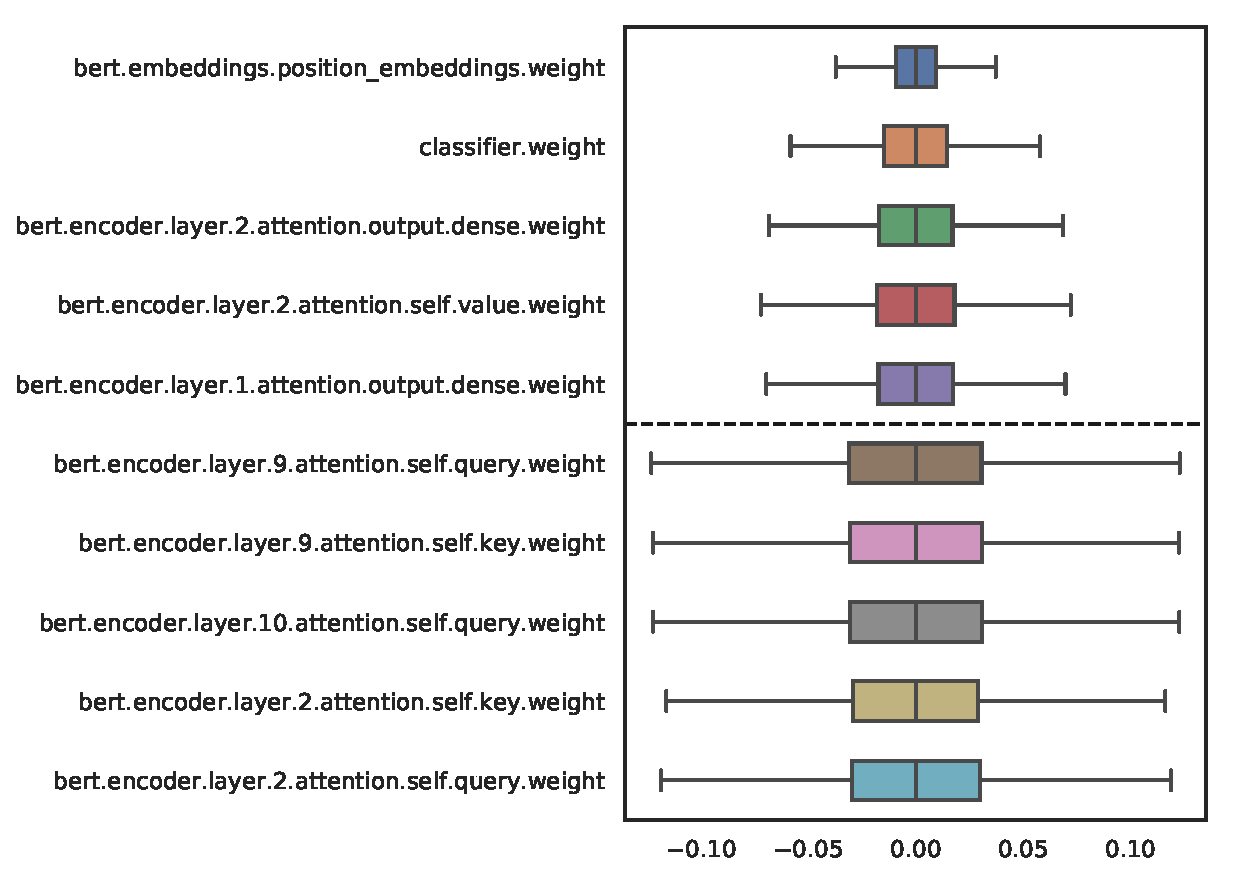
\includegraphics[width=.5\textwidth]{../figs/value_by_layer.pdf}
\caption{Weight distributions for five most/least variable layers}
\label{fig:weightsbylayer}
\end{figure}

Our non-difference distortions are more sensitive to the compression parameter
(whether prune rate or SVD rank). We find it difficult to achieve performance
comparable to the uncompressed BERT with a significantly compressed model. Among
the different distortion methods, we favor pruning for its computational
simplicity, and see no evidence that SVD achieves better compression.

% Things to say about DeepTwist
% \begin{itemize}
%   \item Stratified prune better
%   \item Prune rate mad robust
%   \item Diff gud
%   \item ``Improved performance''
%   \item QQP takes long, but looks okay
%   \item Didn't try only pruning the $\bert$ part
% \end{itemize}
% 
% Things to say about KD
% \begin{itemize}
%   \item it bad
%   \item doesn't work
%   \item LSTM weird/CNN incredibly noisy
%   \item \TODO{compare}
% \end{itemize}

When compared to the performance of a fine-tuned BERT on SST-2, our Knowledge
Distillation results---displayed in \cref{tab:kd_results}---fall short. However,
it is important to note the student networks are also much smaller than BERT. To
isolate the effect of KD, we compare the performance of
\citet{kim2014convolutional}'s CNN trained on the correct labels versus the BERT
probabilities. This suggests a modest performance benefit of two percentage
points in validation accuracy. However, we see no evidence of training being
sped up by using KD.

We also identify some curious behavior in the KD training curves. When training
the LSTM on the BERT outputs, neither training loss nor validation loss decrease
at first. In fact, they stay approximately constant for a couple of epochs. Only
after this prolonged period does loss abruptly start going down, producing a
normal curve from that point forward. We find this---depicted in
\cref{fig:kdlstmloss}---remarkably puzzling. We hypothesize this may be the
effect of our adaptive learning rate starting out too low and taking multiple
epochs to grow to a point where it can meaningfully update parameters. 

\begin{figure*}[tb]
\centering
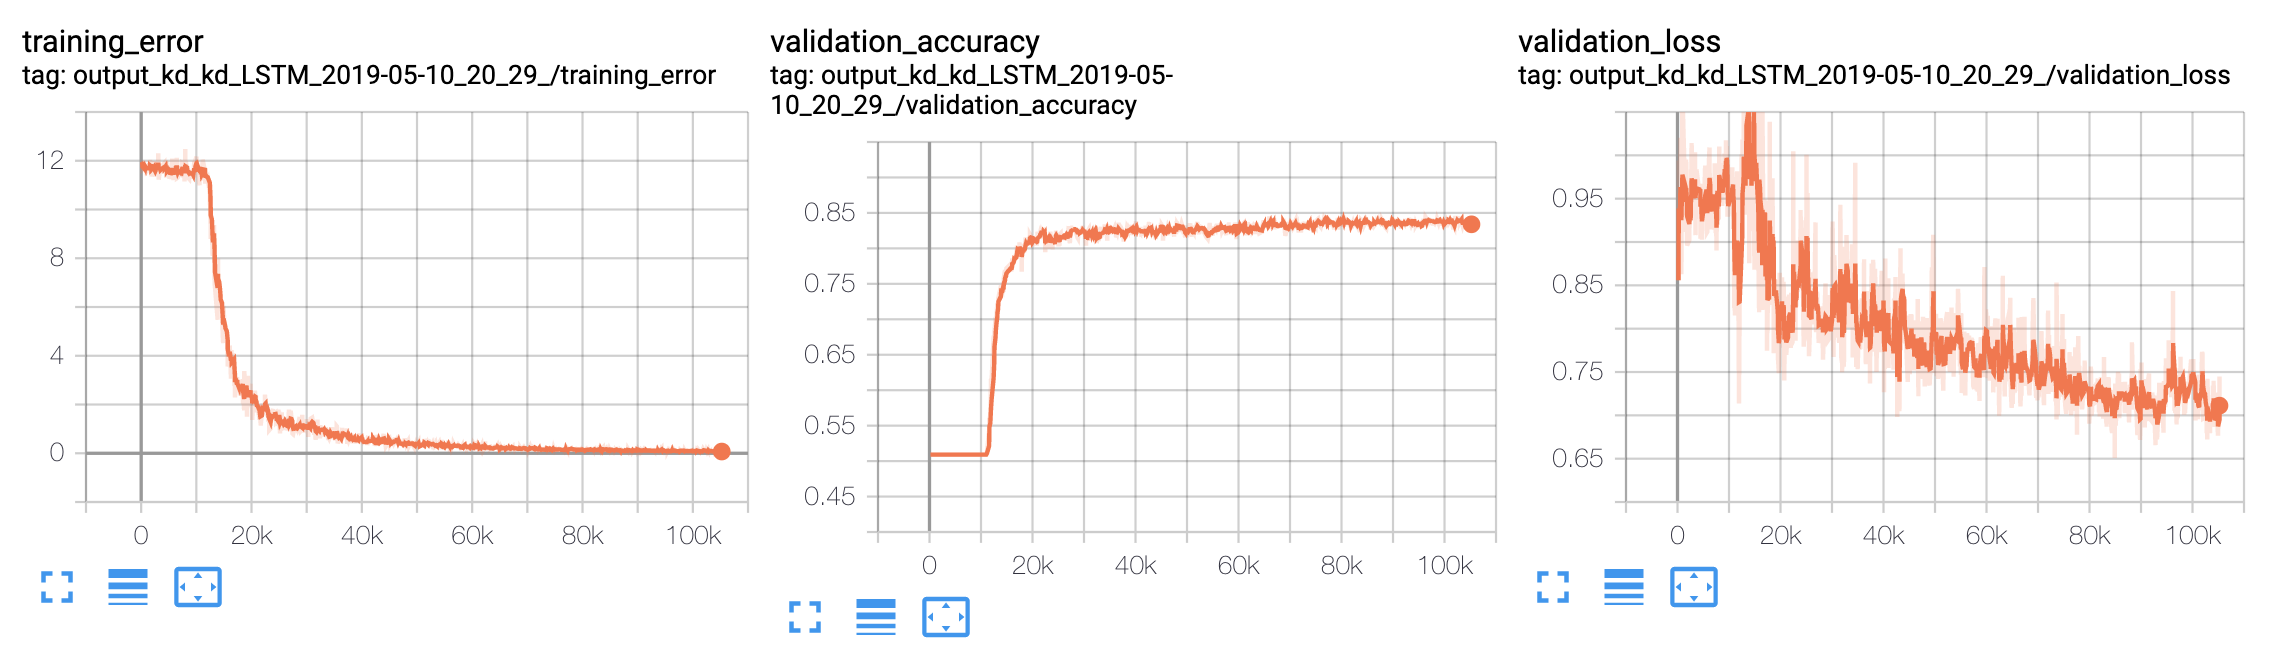
\includegraphics[width=\textwidth]{../figs/kd_lstm_training.png}
\caption{Training loss (left), val. loss (middle), and val. accuracy
(right) for LSTM KD}
\label{fig:kdlstmloss}
\end{figure*}

% \begin{itemize}
% \item What conclusions can you draw from the results section?
% \item Is there further analysis you can do into the results of the system? Here
% is a good place to include visualizations, graphs, qualitative analysis of your
% results.
% 
% \item  What questions remain open? What did you think might work, but did not?
% \end{itemize}



% \begin{figure}
%   \centering
%   \missingfigure{}
%   \missingfigure{}
%   \missingfigure{}
%   \caption{Visualizations of the internals of the system.}
% \end{figure}

\section{Conclusion}

\begin{itemize}
\item What happened?
\item What next?
\end{itemize}



% \section*{Acknowledgements}

% \textbf{Do not} include acknowledgements in the initial version of
% the paper submitted for blind review.

% If a paper is accepted, the final camera-ready version can (and
% probably should) include acknowledgements. In this case, please
% place such acknowledgements in an unnumbered section at the
% end of the paper. Typically, this will include thanks to reviewers
% who gave useful comments, to colleagues who contributed to the ideas,
% and to funding agencies and corporate sponsors that provided financial
% support.


\bibliography{paper}
\bibliographystyle{icml2017}

\end{document}
